\documentclass{beamer}
\usepackage{ulem,amsthm}
\usepackage{tikz}
\usetikzlibrary{arrows}
\title{Design Patterns}
\theoremstyle{definition}

\begin{document}
    \frame{\titlepage}
    \frame{
        \frametitle{Design Patterns}
        \framesubtitle{Introduction Lite}
        Some guys got together and wrote down some $patterns$ they've encountered over their careers in software development and slapped some names on them.
        \begin{center}
            \uncover<2->{\large{That's it... really.}}
        \end{center} 
    }
    \frame{
        \frametitle{Design Patterns}
        \framesubtitle{Introduction Lite}
        \begin{center}
            \theoremstyle{definition}
            \begin{definition}
            Design Patterns are recurring architectural concepts in software development that have been used to solve specific problems.
            \end{definition}
        \end{center}
    }
    \frame{
        \frametitle{Design Patterns}
        \framesubtitle{Introduction Lite}
        \begin{enumerate}
            \item There are many named $patterns$ in the wild.
            \item You've already derived and used a couple patterns.
        \end{enumerate}
    }
    \frame{
        \frametitle{Design Patterns}
        \framesubtitle{Introduction Lite}
        \begin{center}
            You just did not know it was a $thing$ that had a name.
        \end{center}
    }
    \frame{
        \frametitle{Design Patterns}
        \framesubtitle{Introduction Lite}
        \begin{center}
            And they exist everywhere \textbf{else}...
        \end{center}
    }
    \frame{
        \frametitle{Design Patterns}
        \framesubtitle{Learning how to count... again}
        \begin{center}
        Count by $1$'s
        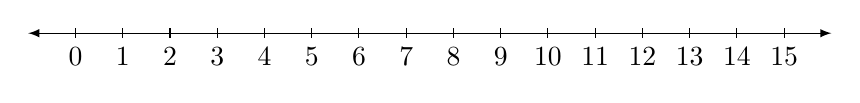
\begin{tikzpicture}[scale=0.60]
            \draw[latex-latex] (-1,0) -- (16,0) ;
            \foreach \x in {0,1,2,3,4,5,6,7,8,9,10,11,12,13,14,15}
                \draw[shift={(\x,0)},color=black](0pt,3pt) -- (0pt,-3pt);
            \foreach \x in {0,1,2,3,4,5,6,7,8,9,10,11,12,13,14,15}
                \draw[shift={(\x,0)},color=black](0pt,3pt) -- (0pt,-3pt) node[below] {$\x$};
        \end{tikzpicture}
        \uncover<2->{Easy right?}
        \end{center}
    }
    \frame{
        \frametitle{Design Patterns}
        \framesubtitle{Learning how to count... again}
        \begin{center}
            What mathematical operation did you use?
        \end{center}
    }
    \frame{
        \frametitle{Design Patterns}
        \framesubtitle{Learning how to count... again}
        \begin{center}
            Now Count by $5$'s 
        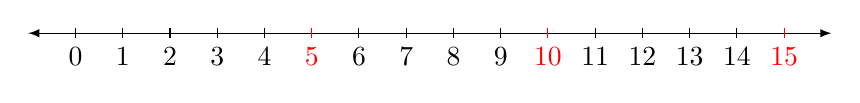
\begin{tikzpicture}[scale=0.60]
            \draw[latex-latex] (-1,0) -- (16,0) ;
            \foreach \x in {0,1,2,3,4,5,6,7,8,9,10,11,12,13,14,15}
                \draw[shift={(\x,0)},color=black](0pt,3pt) -- (0pt,-3pt);
            \foreach \x in {0,1,2,3,4,6,7,8,9,11,12,13,14}
                \draw[shift={(\x,0)},color=black](0pt,3pt) -- (0pt,-3pt) node[below] {$\x$};
            \foreach \x in {5,10,15}
                \draw[shift={(\x,0)},color=red](0pt,3pt) -- (0pt,-3pt) node[below] {$\x$};
        \end{tikzpicture}
        \end{center}
    }
    \frame{
        \frametitle{Design Patterns}
        \framesubtitle{Think like a programmer}
        \begin{center}
            \begin{enumerate}
                \item Create a function that calculates the $nth$ multiple of $5$.
                \item Create a function that calculates the \textit{next} multiple of $5$.
                \item What do all the multiples of $5$ have in common?
            \end{enumerate}
        \end{center}
    }
    \frame{
        \frametitle{Design Patterns}
        \framesubtitle{Think like a programmer}
        \begin{center}
            \begin{definition}
                \textbf{intrinsic state} - sharable features of the defines something.
            \end{definition}
            \uncover<2->{
                \begin{definition}
                    \textbf{extrinsic state} - features/behavior created by a context of usage and therefore can not be shared.
                \end{definition}
            }
        \end{center}
    }
    \frame{
        \frametitle{Design Patterns}
        \framesubtitle{Think like a programmer}
        \begin{center}
            \begin{enumerate}
                \item <1-> What is an \textbf{intrinsic state} of numbers that are multiples of $5$?
                \item <2-> Provide an \textbf{extrinsic state} for a multiple of $5$.
           \end{enumerate}
        \end{center}
    }
    \frame{
        \frametitle{Design Patterns}
        \framesubtitle{Think like a programmer}
        \begin{center}
            \textbf{Task}: Create a \textbf{NumberLine} class that represents the first $77$ trillion multiples of $5$ on the interval $(0, \infty)$
        \end{center}
    }
    \frame{
        \frametitle{Design Patterns}
        \framesubtitle{Flyweight}
        \begin{center}
            A \textbf{flyweight} is a pattern where you can use a single shared object to represent many $items$.
        \end{center}
    }
    \frame{
        \frametitle{Design Patterns}
        \framesubtitle{Flyweight}
        \begin{center}
            \huge{Huh?!}
        \end{center}
    }
    \frame{
        \frametitle{Design Patterns}
        \framesubtitle{Flyweight}
        \begin{center}
            \huge{You already know how to do this in ruby}
        \end{center}
    }
    \frame{
        \frametitle{Design Patterns}
        \framesubtitle{Flyweight}
        \begin{center}
            \sout{Kanye's} Conway's Game of Life
            \begin{enumerate}
                \item why couldn't we create an object for each cell in a $large$ grid?
                \item what was the \textbf{intrinsic state} of a cell?
                \item what was the \textbf{extrinsic state} of a cell?
            \end{enumerate}
        \end{center}
    }
    \frame{
        \frametitle{Design Patterns}
        \framesubtitle{Flyweight}
        \begin{center}
            \textbf{Task}: Create an object or object instance that represents all live cells in a $\infty$-by-$\infty$ sized grid.
        \end{center}
    }
    \frame{
        \frametitle{Design Patterns}
        \framesubtitle{Flyweight}
        \begin{center}
            \Huge{Ta-dah!}
        \end{center}
    }
\end{document}
